\documentclass[]{standalone}
\usepackage{tikz}
\usepackage{tikz-timing}[2009/12/09]{\tiny }
\usetikzlibrary{chains,automata,shapes.multipart,calc,positioning,shapes.geometric,fit}
\usepackage{tikz-qtree}
\usepackage{varwidth}
\usepackage{circuitikz}
\usetikzlibrary{decorations,decorations.pathmorphing,decorations.pathreplacing}


\begin{document}

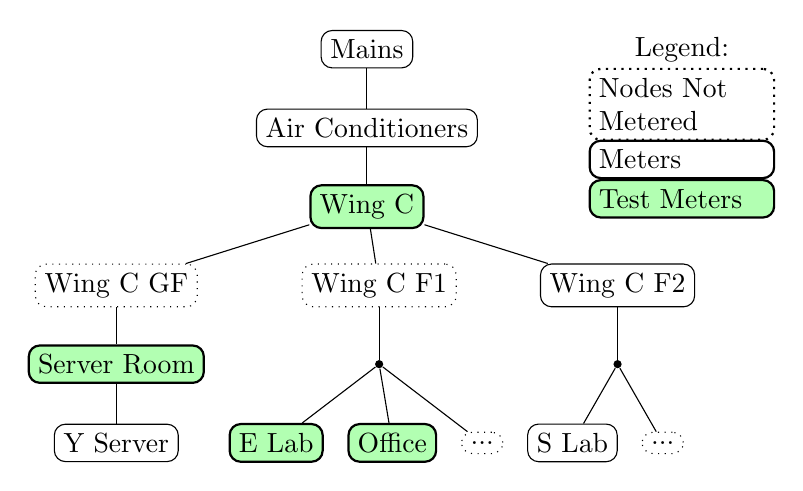
\begin{tikzpicture}[scale= 1.0, every tree node/.style={draw, rectangle,rounded corners,dotted},
level distance=1cm,sibling distance=.3cm, 
edge from parent path={(\tikzparentnode) -- (\tikzchildnode)}]
\Tree [.\node[solid](mains) {Mains}; 
	[.\node[solid] {Air Conditioners};    
		[.\node[fill=green!30,thick,solid] {Wing C};
			[ .\node(gf) {Wing C GF};
				[ .\node[fill=green!30,thick,solid]{Server Room}; 	
				[ .\node[solid]{Y Server}; ]
			]
			]
			[ .{Wing C F1}  
				[ .\node (f1) [draw=none,circle,inner sep=0pt,fill] {.};
					[ .\node[fill=green!30,thick,solid]{E Lab}; ] 
					[.\node[fill=green!30,thick,solid]{Office}; ] 
					[ .{...} ]
                    % [ .{Conf. Room} ]
				] 
			]
			[ .\node[solid] {Wing C F2};
				[ .\node (f2) [draw=none,circle,inner sep=0pt,fill] {.};
				[ .\node[solid] {S Lab}; ]
				[ .{...} ]
				]
			] 
		] 
	]
]
% \node(abc)[red, above of=gf] {Test};
%\node (outer) [draw, fit=(mains) (gf) (f2), blue, rounded corners,text depth=4cm,text height=.3cm,inner sep=5] {Power Distribution Room};
\node(d0) [right of=mains] {};
\node(d1) [right of=d0, node distance=2.0cm] {};
\node(d2) [right of=d1] {Legend:};
\node(d3) [below of=d2,draw ,rectangle,rounded corners, node distance=.7cm,thick,dotted, text width=6em] {Nodes Not Metered};
\node(d4) [below of=d3,draw ,rectangle,rounded corners, node distance=.7cm,thick,solid, text width=6em] {Meters};
\node(d5) [below of=d4, draw ,rectangle,rounded corners, node distance=.5cm,fill=green!30,thick,solid, text width=6em] {Test Meters};
\end{tikzpicture}

\end{document}